\begin{center}
	\tikzset{every picture/.style={line width=0.75pt}} %set default line width to 0.75pt        
	
	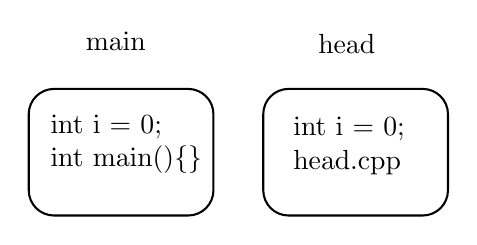
\begin{tikzpicture}[x=0.75pt,y=0.75pt,yscale=-1,xscale=1]
	%uncomment if require: \path (0,300); %set diagram left start at 0, and has height of 300
	
	%Rounded Rect [id:dp31960853174211556] 
	\draw   (225,159.2) .. controls (225,152.46) and (230.46,147) .. (237.2,147) -- (301.8,147) .. controls (308.54,147) and (314,152.46) .. (314,159.2) -- (314,195.8) .. controls (314,202.54) and (308.54,208) .. (301.8,208) -- (237.2,208) .. controls (230.46,208) and (225,202.54) .. (225,195.8) -- cycle ;
	%Rounded Rect [id:dp47295061263468985] 
	\draw   (338,159.2) .. controls (338,152.46) and (343.46,147) .. (350.2,147) -- (414.8,147) .. controls (421.54,147) and (427,152.46) .. (427,159.2) -- (427,195.8) .. controls (427,202.54) and (421.54,208) .. (414.8,208) -- (350.2,208) .. controls (343.46,208) and (338,202.54) .. (338,195.8) -- cycle ;
	
	% Text Node
	\draw (251,118) node [anchor=north west][inner sep=0.75pt]   [align=left] {main};
	% Text Node
	\draw (363,119) node [anchor=north west][inner sep=0.75pt]   [align=left] {head};
	% Text Node
	\draw (234,158) node [anchor=north west][inner sep=0.75pt]   [align=left] {int i = 0;\\int main()\{\}};
	% Text Node
	\draw (351,159.2) node [anchor=north west][inner sep=0.75pt]   [align=left] {int i = 0;\\head.cpp};
	
	
	\end{tikzpicture}
\end{center}